\chapter{Quantum correlations in the weakly-interacting Bose gas}

\NOTE{TOUT CECI EST MAL ECRIT}

One of the key and on-going challenges of quantum mechanics is to understand macroscopic systems containing a large number of particles $N$, commonly referred as many-body physics. Trying to consider all the possible degrees of freedom of each individual particle and interactions effects would result in an incredibly complex problem impossible to solve theoretically. Studying such systems thus require to use approximations ...

Physicists were able to describe a gas of a large number of bosonic particles with increasing complexity throughout history. The first step was the development of statistical physics, aiming to build a bridge between the microscopic properties of individual atoms or molecules and macroscopic properties of bulk materials described by thermodynamics. This approach culminated in the theory of the ideal Bose gas, ideal meaning here that all particles are non-interacting. This theory found great success with the notable prediction of a new state of matter, the Bose-Einstein condensate. 

The next step was then to increase the complexity of the problem by adding interactions between the particles. ...

While also greatly successful, the mean-field approach neglects by essence interaction phenomena between individual particles. To characterize such effects, we thus need to go beyond the mean-field approximation. \NOTE{c'est bien nul je laisse pour l'instant}




\section{Correlation functions}

\subsection{First order correlation function of light}

Let us begin our journey with correlation functions with the simple example of the classical description of light. Correlation functions of light were developed in strong connection with the notion of \textbf{coherence} characterizing the possibility for waves to interfere. A light field is said to be coherent when there is a fixed phase relationship for the electric field at different positions (spatial coherence) and different times (time coherence). 


\begin{figure}
    \centering
    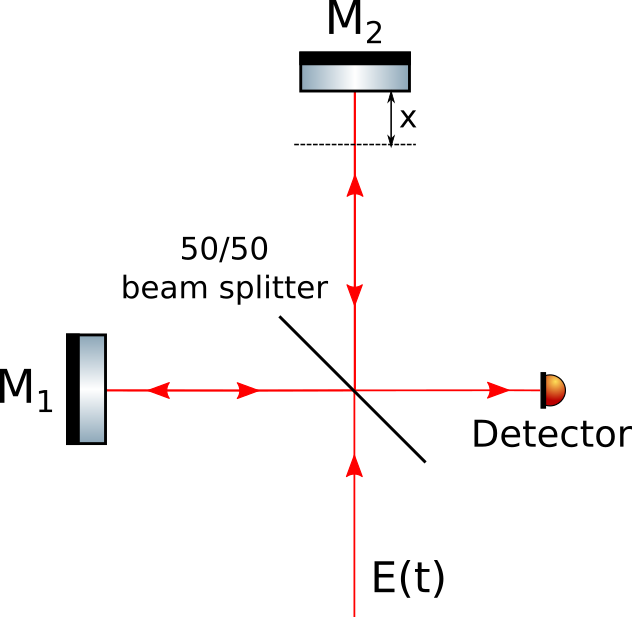
\includegraphics[width=0.55\textwidth]{Fig/Chapter1/michelson.png}
    \caption{Principle of the Michelson interferometer.}
    \label{fig:michelson}
\end{figure}


To illustrate where correlation functions come from, let us begin by taking a look at time coherence in the emblematic Michelson interferometer (see Fig.-\ref{fig:michelson}). We send at the input of the interferometer a complex light field $E(t)$. The intensity measured by the detector writes:

\begin{equation}
    I=\mean{\abs{E(t)+E(t-\tau)}^2}
    \label{eq:i_michelson}
\end{equation}

where $\mean{...}$ denotes the time average made by the detector and $\tau=\frac{2x}{c}$ the delay between the two interfering waves induced by the optical path difference between the two arms of the interferometer. Developing equation \ref{eq:i_michelson} we get:

\begin{equation}
    I=\mean{\abs{E(t)}^2} + \mean{\abs{E(t-\tau)}^2} + 2 {\rm{Re}} \mean{E(t) E^*(t-\tau)}
\end{equation}

For simplicity sake, let's assume that the source is stationary to write $\mean{\abs{E(t)}^2} = \mean{\abs{E(t-\tau)}^2} = I_0$, we then obtain :

\begin{equation}
    I= 2 I_0 (1 + {\rm{Re}} (g^{(1)} (\tau))) \ , \ g^{(1)} (\tau) = \frac{ \mean{E(t) E^*(t-\tau)}}{\mean{\abs{E}^2}}
\end{equation}

We have introduced the normalized \textbf{first-order correlation function} $g^{(1)}$ that characterizes the interference term. If $E(t)$ and $E(t-\tau)$ are independent and thus uncorrelated, $\mean{E(t) E^*(t-\tau)} = \mean{E(t)} \mean{ E^*(t-\tau)}=0$ and interference cannot be observed \NOTE{corriger}. On the other hand, if there is a \textbf{correlation} between these two quantities, an interference phenomenon can be observed. The same reasoning can be conducted for the spatial coherence for instance with the non less famous Young double slit experiment. 

We will not detail here all the intricacies of the study of first-order correlation functions for different light sources. The main point to remember is that the first order correlation function is a natural way to characterize the coherence properties of a light source, and thus its ability to produce interferences. 





\subsection{Classical example : HBT with chaotic light}

\subsection{HBT with the perfect Bose gas}

\section{Bogoliubov theory of the weakly-interacting gas}

Thus far, we have familiarized ourselves with correlation functions and seen through a few examples the kind of information they contain. We will now try to use this tool to study a many-body problem, the weakly-interacting homogeneous Bose gas, {\it i.e.} an ensemble of bosonic particles with weak contact interactions in a box of volume $V$. The theoretical description of this system has been developed by Nikolay Bogoliubov in his famous 1947 article \cite{bogoliubov1947}. In this section, we will remind the main lines of Bogoliubov's approach and see what it tells us in terms of correlation functions.

\subsection{Bogoliubov approximation}

\NOTE{Etapes avant?}

The Hamiltonian of the weakly-interacting Bose gas with contact interactions writes:

\begin{equation}
    \hat{H}=\sum_{\bm{k}}\frac{\hbar^2 k^2}{2m} \hat{a}^{\dagger}_{\bm{k}}  \hat{a}_{\bm{k}} +  \frac{g}{2V} \sum \hat{a}^{\dagger}_{\bm{k_1}+\bm{k_3}} \hat{a}^{\dagger}_{\bm{k_2}-\bm{k_3}} \hat{a}_{\bm{k_1}} \hat{a}_{\bm{k_2}} 
\end{equation}

\noindent where $g=\dfrac{4 \pi \hbar^2 a_s}{m}$ is the strength of the interactions with $a_s$ the s-wave sacttering length. \NOTE{DILUTENESS?} In order to simplify this Hamiltonian, we use the Bogoliubov approximation that relies on two points:

\begin{itemize}
    \item Since the interactions are weak, we assume that the number of atoms outside of the BEC is small. We therefore only consider interaction processes removing two particles from the BEC or bringing back two particles into the BEC. Mathematically speaking, we drop all terms higher than quadratic in $\hat{a}_{\bm{k}}$ and $\hat{a}^{\dagger}_{\bm{k}}$.
    \item The number of atoms $\NBEC$ is assumed to be very large. Therefore, we replace $\hat{a}_{\bm{0}}$ and $\hat{a}^{\dagger}_{\bm{0}}$ by $\sqrt{\NBEC}$. 
\end{itemize}

With these approximation, the simplified Hamiltonian writes:

\begin{equation}
    H_{\rm{bogo}}=\sum_{\bm{k}}\frac{\hbar^2 k^2}{2m} a^{\dagger}_{\bm{k}}  a_{\bm{k}} +  \frac{gn}{2} \sum_{\bm{k}} (a^{\dagger}_{\bm{k}} a^{\dagger}_{-\bm{k}} +a_{\bm{k}} a_{-\bm{k}})+\frac{gn\NBEC}{2}
\end{equation}

What we now want to is diagonalize the Hamiltonian. This is achieved through the linear Bogoliubov transformation where we introduce a new operator:

\begin{equation}
    \hat{b}_{\bm{k}}=u_{\bm{k}} \hat{a}_{\bm{k}} + v_{-\bm{k}} \hat{a}^{\dagger}_{-\bm{k}}
\end{equation}

To determine the expression of the coefficients $u_{\bm{k}}$ and $v_{\bm{k}}$, we impose that the new operator $\hat{b}_{\bm{k}}$ follows the bosonic operator commutation rule:

\begin{equation}
    [\hat{b}_{\bm{k}},\hat{b}^{\dagger}_{\bm{k}'}]= \delta_{\bm{k},\bm{k}'}
\end{equation}

This gives $u_{\bm{k}}^2 -  v_{-\bm{k}}^2 =1$. We can therefore write $u_{\bm{k}}={\rm cosh}(\alpha_{\bm{k}})$ and $v_{-\bm{k}}={\rm sinh}(\alpha_{\bm{k}})$ and look to determine $\alpha_{\bm{k}}$. This value must be chosen so that the coefficients of the terms in $\hat{b}^{\dagger}_{\bm{k}} \hat{b}^{\dagger}_{-\bm{k}}$ and $\hat{b}_{\bm{k}} \hat{b}_{-\bm{k}}$ vanish. We obtain an additional equation:

\begin{equation}
    \frac{g n}{2}\left(u_{\bm{k}}^{2}+v_{-\bm{k}}^{2}\right)+\left(\frac{k^{2}}{2 m}+g n\right) u_{\bm{k}} v_{-\bm{k}}=0
\end{equation}

from which we finally obtain after a few calculations using the properties of hyperbolic functions:

\begin{equation}
    u_{\bm{k}}, v_{-\bm{k}}=\pm\left(\frac{\hbar^2k^{2} / 2 m+g n}{2 \varepsilon(k)} \pm \frac{1}{2}\right)^{1 / 2}
\end{equation}

with 

\begin{equation}
    \varepsilon(k)=\sqrt{\frac{\hbar^2 k^2}{2m}(\frac{\hbar^2 k^2}{2m}+2gn)}
\end{equation}

the famous Bogoliubov dispersion relation. The Hamiltonian has now been diagonalized and writes:

\begin{equation}
    \hat{H}_B = \sum_{\bm{k}}\varepsilon(k) b^{\dagger}_{\bm{k}}  b_{\bm{k}}+E_0
\end{equation}

The system of interacting particles has thus been transformed into a system of non-interacting Bogoliubov quasi-particles associated to creation and annihilation operators $\hat{b}^{\dagger}_{\bm{k}}$ and $\hat{b}_{\bm{k}}$ with a dispersion relation $\varepsilon(k)$. The prediction of this excitation spectrum is one of the key results of Bogoliubov theory that we will now discuss in further details.

\subsection{Spectrum of excitations}

The Bogoliubov dispersion relation has two clear asymptotic trends for small and high momentum values. For low values of $k$, using $\frac{\hbar^2 k^2}{2m} \ll 2gn$, we obtain:

\begin{equation}
    \varepsilon(k) \underrel{k \to 0}{=} \hbar k \sqrt{\frac{gn}{m}}
\end{equation}

The dispersion relation takes a phonon-like linear dispersion form where the sound velocity is $c=\sqrt{\dfrac{gn}{m}}$. In this regime, the Bogoliubov quasi-particles are thus phonons that can be sen as a coherent superposition of a forward and backward propagating real particles $\hat{b}_{\bm{k}}=u_{\bm{k}} \hat{a}_{\bm{k}} + v_{-\bm{k}} \hat{a}^{\dagger}_{-\bm{k}}$ with $\abs{u_{\bm{k}}} \simeq \abs{v_{-\bm{k}}}$.

On the other hand, at high values of $k$, the dispersion relation becomes the one of free particles:

\begin{equation}
    \varepsilon(k) \underrel{k \to +\infty}{=} \frac{\hbar^2 k^2}{2m}
\end{equation}

In terms of operators, $v_k \underrel[c]{k \to +\infty}{=} 0$ and $u_k \underrel[c]{k \to +\infty}{=} 1$ so $\hat{b}_{\bm{k}}\underrel[c]{k \to +\infty}{=}\hat{a}_{\bm{k}}$, a quasi-particle is equivalent to a real particle. 

The transition between the two regimes occurs when $\frac{\hbar^2 k^2}{2m} \simeq gn$, it thus convenient to define a characteristic length associated to this momentum range:

\begin{equation}
    \xi = \sqrt{\frac{\hbar^2}{2mgn}}
\end{equation}

This length is called the \textbf{healing length} \NOTE{COMPLETER?}. We will use it later when discussing our experimental results to characterize the region of the Bogoliubov spectrum we are probing.

The Bogoliubov spectrum of excitation has been a very successful theoretical prediction observed experimentally in a large variety of systems \cite{miller1962, steinhauer2002excitation, ozeri2005, fontaine2018, stepanov2019}. However, the Bogoliubov theory also gives an additional prediction for the \textbf{ground-state} of the system.

\begin{figure}
    \centering
    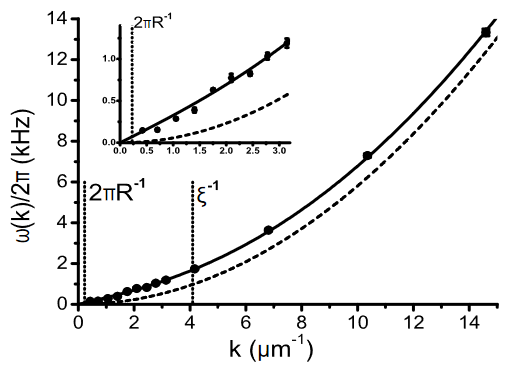
\includegraphics[width=0.65\textwidth]{Fig/Chapter1/bogo_steinhauer.png}
    \caption{Experimental observation of the Bogoliubov excitation spectrum (Steinhauer {\it et al.} \cite{steinhauer2002excitation}). The phononic and free particle parts are clearly identifiable. The inset shows a zoom on the linear part of the spectrum and the dashed the free particle spectrum. $\xi$ is the healing length of the condensate.}
    \label{fig:my_label}
\end{figure}

\subsection{The quantum depletion}

As we have just seen, the Bogoliubov approach describes the weakly-interacting Bose gas excitations as non-interacting quasi-particles. They therefore behave as ideal bosons and follow the Bose distribution:

\begin{equation}
    \langle b^{\dagger}_{\bm{k}}  b_{\bm{k}} \rangle=\frac{1}{e^{-\varepsilon(k)/(k_B T)}-1} 
\end{equation}

Naturally, at $T=0$, the population of quasi-particles is null: $\langle b^{\dagger}_{\bm{k}}  b_{\bm{k}} \rangle_{T=0}=0$. That being said, let us now write the population of real particles for a given momentum $k \neq 0$:

\begin{equation}
    \langle a^{\dagger}_{\bm{k}}  a_{\bm{k}} \rangle=\textcolor{blue}{(|u_k|^2+|v_k|^2)\langle b^{\dagger}_{\bm{k}}  b_{\bm{k}} \rangle} + \textcolor{green}{|v_k|^2}
\end{equation}

The blue term corresponds to the Bogoliubov excitations populated by temperature. We will call the fraction of particles removed from the condensate this way the \textcolor{blue}{\textbf{thermal depletion}}. This fraction vanishes at $T=0$. Very interestingly, we see the apparition of an additional term \textcolor{green}{$|v_k|^2$} that results from the non commutation of the bosonic creation and annihilation operators, the signature of an essentially quantum phenomenon. This term tells us that $\langle a^{\dagger}_{\bm{k}}  a_{\bm{k}} \rangle_{T=0} \neq 0$, meaning that there are some atoms outside of the BEC with a non zero momentum in the ground state! Under the interplay between interactions and quantum fluctuations, some atoms are removed from the BEC and obtain a non zero momentum. The fraction of these atoms is called the \textcolor{green}{\textbf{quantum depletion}}. 

We are thus looking at a system which seems to fall into our general area of interest described in the introduction of this thesis, namely many-body systems with interactions displaying quantum behaviors. The weakly-interacting Bose gas shows the advantage to be one of the conceptually simplest many-body systems for which a theory can be derived as we just have shown. As explained in the beginning of this chapter, many-body systems are often efficiently characterized by correlation functions. Let us now discuss what are the relevant correlation functions to study for the weakly-interacting Bose gas.

\section{Hanbury Brown and Twiss effect with interacting atoms}


\section{k/-k correlations in the many-body ground-state}

Let us now come back to the ground-state of the weakly-interacting Bose gas and the quantum depletion. We will now try to build a microscopic, physically meaningful picture of how the quantum depletion emerges. We remind that a key ingredient of the Bogoliubov theory is that the only considered interaction processes are the ones involving two particles of the BEC or two particles outside of the BEC being brought into it. From this consideration, we understand that the atoms belonging to the quantum depletion were initially in the BEC and were removed from it after undergoing a two-body interaction process. The interaction process populating the quantum depletion thus involves two atoms in the BEC with a momentum $k \simeq 0$. To conserve the overall momentum, the two atoms leaving the BEC then have opposite momenta $\bm{k}$ and $-\bm{k}$ and form a momentum correlated pair. This falls exactly into the kind of signal we are interested in, namely correlations between several particles, here two, caused by a quantum, interaction-induced effect.

The common factor with quantum effects is that they usually defy our intuition built on our observation of the everyday world, well described by classical physics. In this case, the "quantum weirdness" comes from the fact this process seems to violate the conservation of energy: the two at atoms initially at rest each have an extra kinetic energy $\frac{\hbar^2 k^2}{2m}$ after the interaction process giving them the $\bm{k}$ and $-\bm{k}$ momenta. Naturally, the conservation of energy is still well respected here. The apparent contradiction comes from the fact that it is conceptually wrong to isolate two atoms in the BEC. The ground-state must rather be understood as a single many-body wave-function describing indistinguishable atoms, with a non zero component for momentum values $k \neq 0$. The energy of the many-body ground state of the weakly-interacting Bose gas contains a small correction that corresponds to the presence of the \kmk pairs of the quantum depletion. This small correction is called the Lee-Huang-Yang correction, named after the authors of the seminal 1957 article \cite{lee1957} that first predicted the presence of the \kmk pairs.

Although being more than 60 years old, the prediction of the presence \kmk correlations in the ground-state of a weakly interacting Bose gas still lacks an experimental observation of the microscopic \kmk pairing. This will be the main objective and central theme of this thesis. \NOTE{RAJOUTER UN TRUC SUR HAWKING TOUSSA ?}

Observing such a correlation signal requires some key experimental ingredients. The principal one is to have an experiment capable of measuring the momentum of individual atoms in momentum space and not only the momentum density as in most cold atoms experiment. This will be the subject of Chapter 3. In addition, there are several key features of the \kmk correlation signal that we need to properly understand to design an experimental scheme where the \kmk correlation signal can be properly detected.

\subsection{Momentum spread of the quantum depletion}

\subsection{Finite temperature effects}

